\documentclass[10pt, conference, a4paper, final]{IEEEtran}
\IEEEoverridecommandlockouts
% For better handling of math expressions
\usepackage{amsmath}

% For better formatting of lists
\usepackage{enumitem}

% Optional for improved typography
\usepackage{microtype}
\usepackage[margin=1in]{geometry} % Adjust margins as needed
\usepackage{lipsum} % Provides sample text. Remove this for your actual document.
\usepackage[table,xcdraw]{xcolor}
\usepackage{colortbl}
\usepackage{graphicx} % Required for including images
\usepackage{graphicx}
\usepackage{textcomp}
\usepackage{xcolor}
\usepackage{float}
\usepackage{amsmath}
\usepackage{longtable}
\usepackage{booktabs}
\usepackage{multicol}
\usepackage{multirow}
\usepackage{relsize, fullpage, url, array}
\usepackage{lscape, afterpage}
\usepackage{float,lscape}
\usepackage{algorithm}
\usepackage{algorithmic}  
\usepackage[algo2e]{algorithm2e} 
\usepackage{amsmath}
\usepackage{mathtools}
\usepackage{tabularx}
\usepackage{algorithmic}
\usepackage{graphicx}
\usepackage{textcomp}
\usepackage{xcolor}
\usepackage{subcaption}

\title{Enhancing Deep Learning Robustness: A Multidimensional Approach Against Adversarial Threats}
\author{Arooj Arif}
\date{\today} % You can also specify a date manually

\begin{document}

\maketitle % This command creates the title


\begin{abstract}
    One of the key issues in the realm of deep learning involves the lack of transparency 
    in the decision-making processes of AI models, particularly when they encounter attacks 
    intended to deceive them. Modern study struggles with the challenge of hitting an optimal 
    balance between the complexity required for AI models to be effective and the simplicity 
    needed for understanding, which can sometimes result in vulnerabilities within AI systems. 
    Our paper presents an innovative method in artificial intelligence to tackle this important
     issue. To the best of our knowledge, this is the first time Explainable AI (XAI) has been 
     applied to enhance the dependability of deep learning models against these misleading attacks
      by analysing the most crucial areas of images (referred to as vital pixels). 
      To evaluate and comprehend these threats, we employ a cutting-edge set of approaches along 
      with a well-known AI model called a Convolutional Neural Network (CNN). 
      One important aspect of our work is the application of SHAP analysis, a technique 
      that allows us to identify the areas of an image that have the most impact on the AI's 
      predictions. By concentrating on these crucial pixels, we can gain a better understanding 
      of how to strengthen and deceive AI algorithms. Our in-depth research reveals new information 
      about how to strengthen and dependable AI models. This work is a step forward in addressing 
      the present AI security concerns and enhancing the trustworthiness and understandability 
      of AI systems, which is particularly important in cases when precise AI judgements are 
      critical.



\end{abstract}
\section{Introduction}
In the rapidly evolving domain of artificial intelligence, ensuring the robustness of deep learning models against adversarial 
threats has become a critical area of focus. These adversarial attacks, characterized by subtle yet deliberate alterations in the 
input data, pose a significant challenge to the reliability and security of AI systems. Deep learning models, especially Convolutional
 Neural Networks (CNNs), are particularly susceptible to these attacks, despite their otherwise powerful capabilities. This vulnerability
necessitates the development of robust defense mechanisms to secure these systems against such threats 
\cite {Akhtar, McInnes}
Our study introduces a comprehensive approach that blends the strengths of pre-trained CNNs with advanced adversarial simulations, 
SHAP (SHapley Additive exPlanations) analysis, and Explainable AI (XAI) signatures. This multifaceted strategy aims to not only bolster
 the robustness of deep learning models but also to shed light on their decision-making processes. By doing so, it addresses the critical
  need for systems that are secure against adversarial threats and are also transparent in their functioning  \cite {Lee, Morris, Croce}.
The integration of SHAP analysis and XAI is pivotal in this context. These techniques allow for a more nuanced interpretation of complex models, 
enhancing their transparency. This aspect is increasingly vital in applications with high stakes, such as healthcare, where the accuracy and 
explainability of AI decisions are paramount, and in autonomous systems, where safety and reliability are crucial \cite {Zhou}. 
The recent research by \cite {Zhou}, which explores adversarial attacks in the context of IoT network intrusion detection, aligns closely with our work's emphasis on robust and interpretable AI systems.
Furthermore, our proposed methodology undergoes rigorous validation through various case studies. These studies demonstrate the method's effectiveness in 
identifying and mitigating adversarial threats, thereby making a significant contribution to the field of AI security. By highlighting the intrinsic
 connection between model robustness and explainability, our research advances the understanding of how AI systems can be made both secure and interpretable, 
 a balance that is often challenging to achieve but is crucial for the wide-scale adoption of AI technologies.
In summary, this research not only responds to the existing challenges in AI security highlighted by \cite {Akhtar} and \cite {Dong}  but also builds 
upon recent advancements in the field, such as the work of \cite {Morris} and \cite {Croce}, to propose a novel, effective solution for enhancing the robustness and transparency of deep learning systems.
\section{Proposed Methodology:}

\begin{figure*}[!ht]
    \centering
    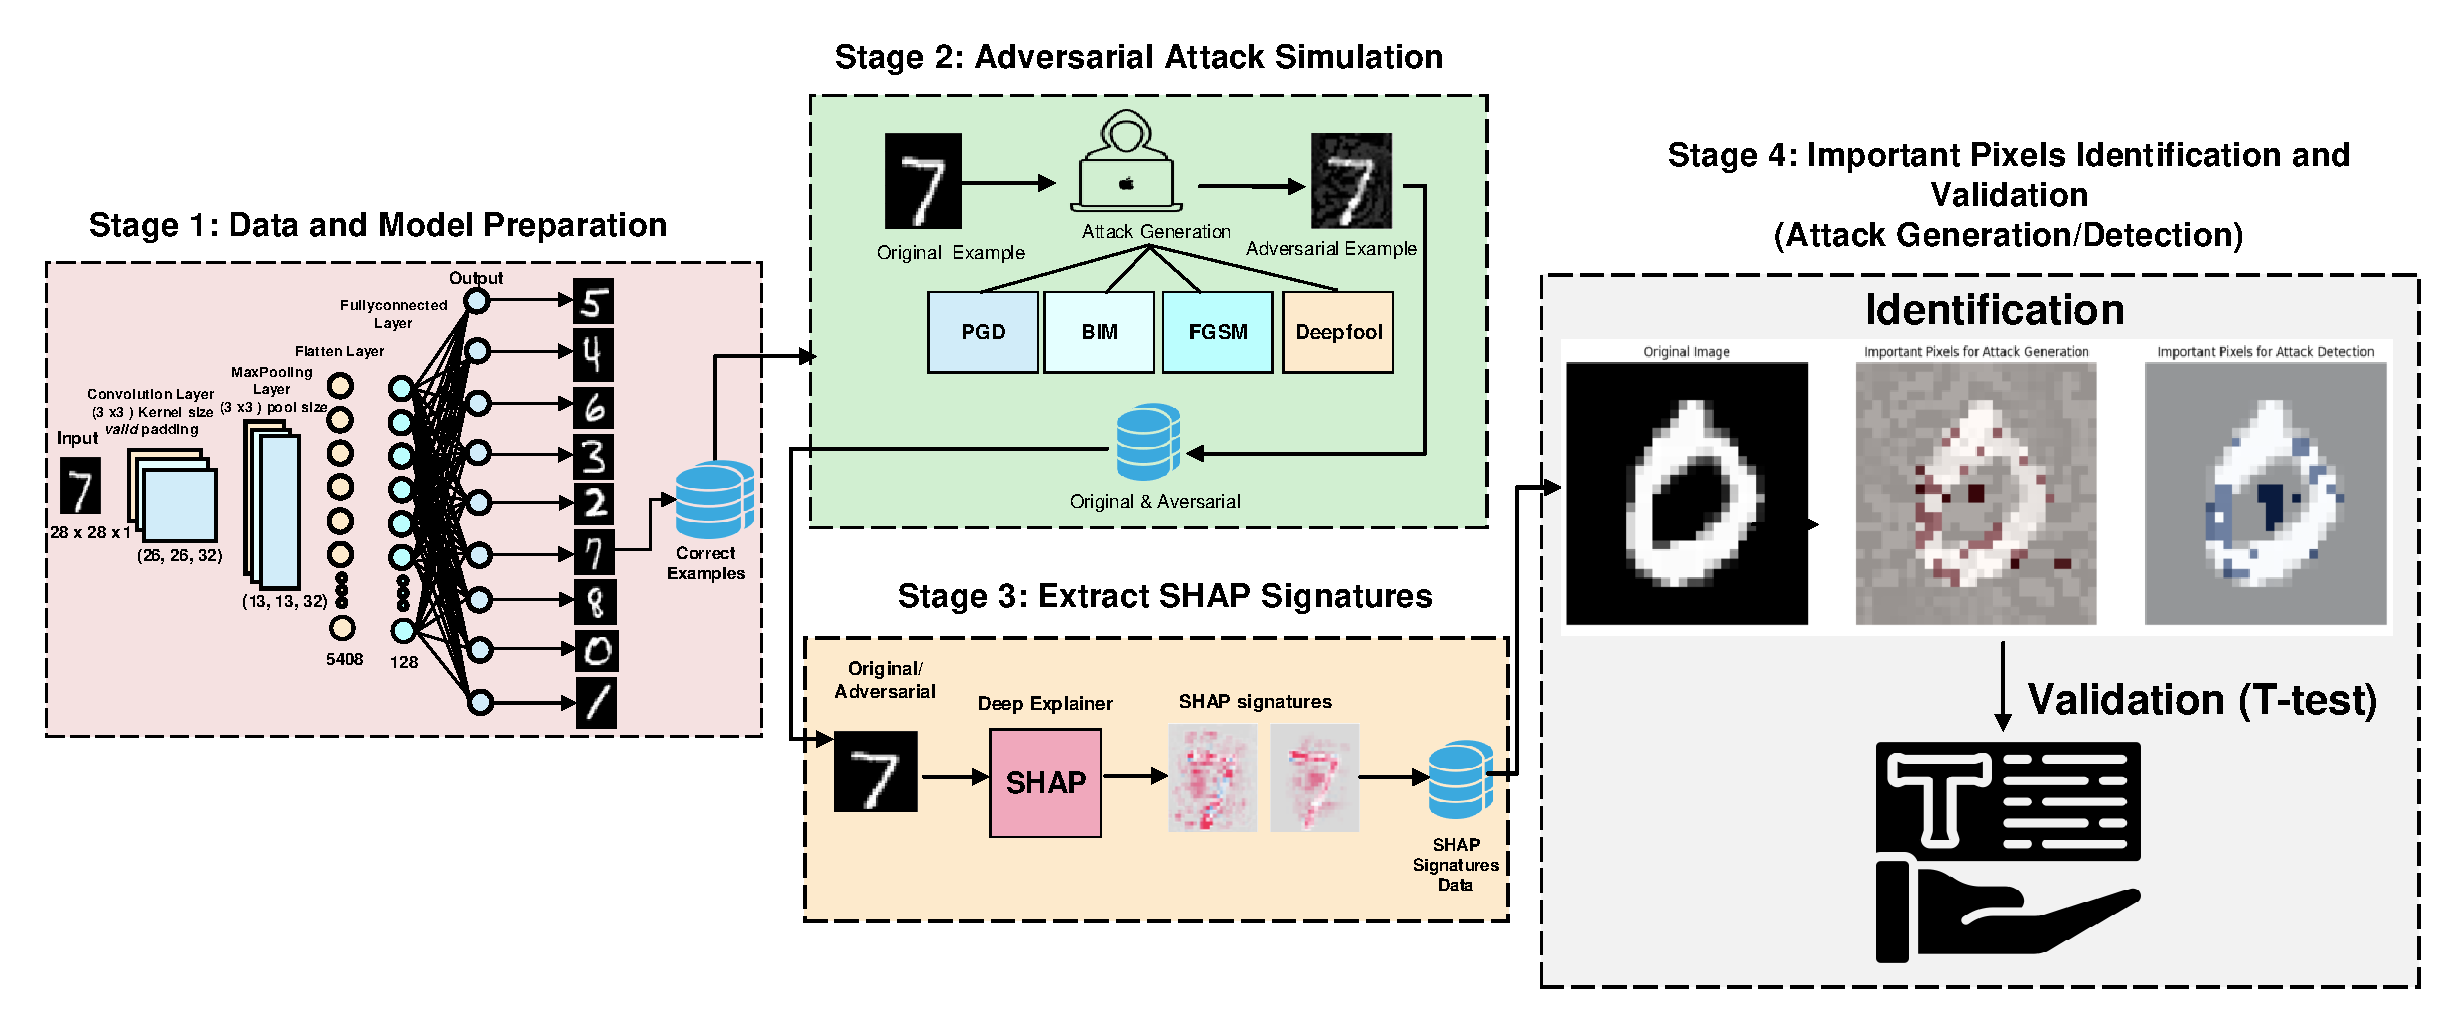
\includegraphics[width=1\textwidth]{paper_images/papermodel_v2.pdf}
    \caption{Overview of the Proposed Model}
    \label{overview}
\end{figure*}
   
Our proposed model, depicted in the Figure. \ref{overview}, is designed to enhance the robustness of deep learning systems against adversarial attacks. It starts with a pre-trained Convolutional Neural Network on the MNIST dataset, focusing on accurate feature extraction. The model then undergoes rigorous adversarial attack simulations using various techniques to assess its resilience. This is followed by an in-depth SHAP analysis to understand pixel-level influences on the model's decisions. The final stage involves employing XAI signatures for binary classification, distinguishing between original and adversarial inputs. This multi-stage approach ensures a comprehensive and robust defense against adversarial threats in machine learning models.

\section{Stage 1: Data and Model Preparation}
In the preliminary phase of our investigation, we utilized a Convolutional Neural Network (CNN), pre-trained on the MNIST dataset, for digit classification. The CNN's established proficiency in feature extraction from image data was crucial for our experiment. A key preprocessing step involved selecting examples that were correctly classified by the model, creating a dataset of accurately predicted instances. This approach aimed to isolate the effects of adversarial perturbations on an otherwise accurately performing model.

The dataset, post-selection, presented a varied class distribution: 973 instances of label 0, 1133 of label 1, 1016 of label 2, 989 of label 3, 969 of label 4, 882 of label 5, 937 of label 6, 1005 of label 7, 946 of label 8, and 984 of label 9. Although not perfectly balanced, this distribution mirrors the natural frequency of digit occurrences in the real world, lending a degree of ecological validity to our study. Acknowledging this slight imbalance was vital for the integrity of our research. It allowed us to critically assess the model's robustness against adversarial attacks in a realistic setting, rather than in an artificially balanced environment.

By focusing on accurately classified instances, we ensured that our subsequent analysis concentrated on the impact of adversarial attacks on an already competent model. This methodical approach to data selection set a clear and realistic groundwork for our investigation, enabling us to explore the resilience of neural networks to adversarial manipulations in a context that closely resembles practical applications.
Objective: Set up the foundational elements for analysis.
Key Actions:
Load the pre-trained MNIST model.
Load and preprocess the dataset, including correct examples and labels.
Assess the model's baseline accuracy on clean data.
\section{Stage 2: Adversarial Attack Simulation}

\subsection{Objective}
The objective of this stage was to rigorously evaluate the model's robustness by generating adversarial examples. This evaluation is essential to understanding how the neural network model performs under manipulated conditions designed to deceive it.

\subsection{Rationale for Epsilon Values}

A critical aspect of our methodology was the selection of epsilon values, \( \varepsilon = [0.03,0.04,0.05,0.1, 0.2, 0.25] \). These values were chosen to represent a spectrum of perturbation intensities:

\begin{itemize}
    \item \textbf{Lower Epsilon Values (\( \varepsilon = 0.03, 0.04, 0.05 \))}: Represent subtle but potentially effective perturbations, testing the model's sensitivity to minimal adversarial modifications.
    
    \item \textbf{Moderate Epsilon Value (\( \varepsilon = 0.1 \))}: Offers a balanced perspective, providing insights into the model's performance under a moderately strong attack.
    
    \item \textbf{Higher Epsilon Values (\( \varepsilon = 0.2, 0.25 \))}: Examine the model's resilience against more aggressive and noticeable adversarial manipulations.
\end{itemize}

The selection of these values allowed for a comprehensive analysis of the model's behavior under varying degrees of adversarial intensity, which is crucial in understanding its overall robustness.

\subsection{Key Actions}
\begin{itemize}
    \item \textbf{Integration of Foolbox for Adversarial Attack Generation:} Utilized Foolbox, a Python library, to facilitate the generation of a wide range of adversarial attacks.
    
    \item \textbf{Implementation and Conduct of Various Adversarial Attacks:} Executed a series of adversarial attacks, including LinfBasicIterativeAttack (BIM), LinfFastGradientAttack (FGSM), LinfDeepFoolAttack, and LinfProjectedGradientDescentAttack (PGD).
    
    \item \textbf{Collection and Analysis of Adversarial Examples:} Systematically collected and analyzed the adversarial examples generated from these attacks.
\end{itemize}\subsection{Inclusion of the UMAP visualization:}

\begin{figure*}[!ht]
    \centering
    \begin{subfigure}{.31\textwidth}
        \centering
        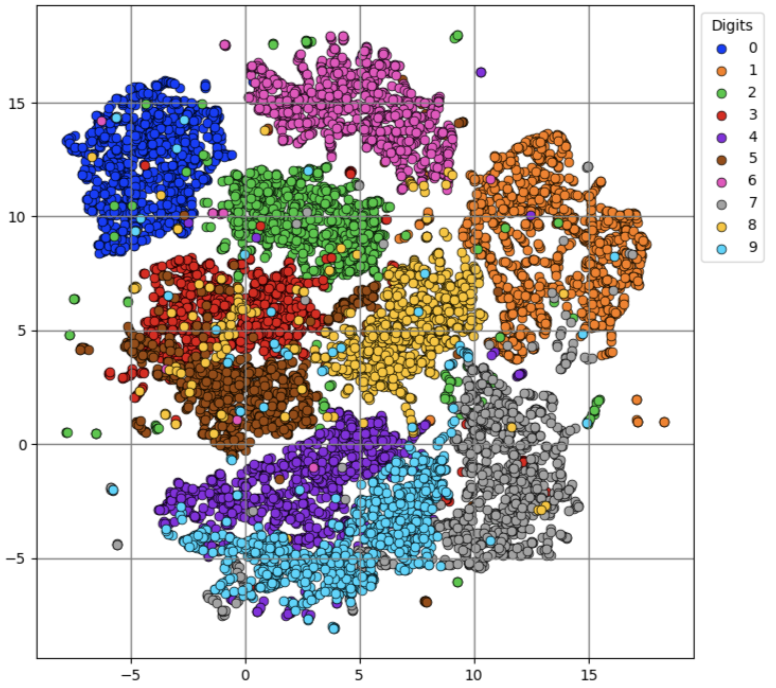
\includegraphics[width=\linewidth]{paper_images/UMAP_mnist.png}
        \caption{Original MNIST digit classes}
        \label{fig:umap_original}
    \end{subfigure}%
    \hfill
    \begin{subfigure}{.34\textwidth}
        \centering
        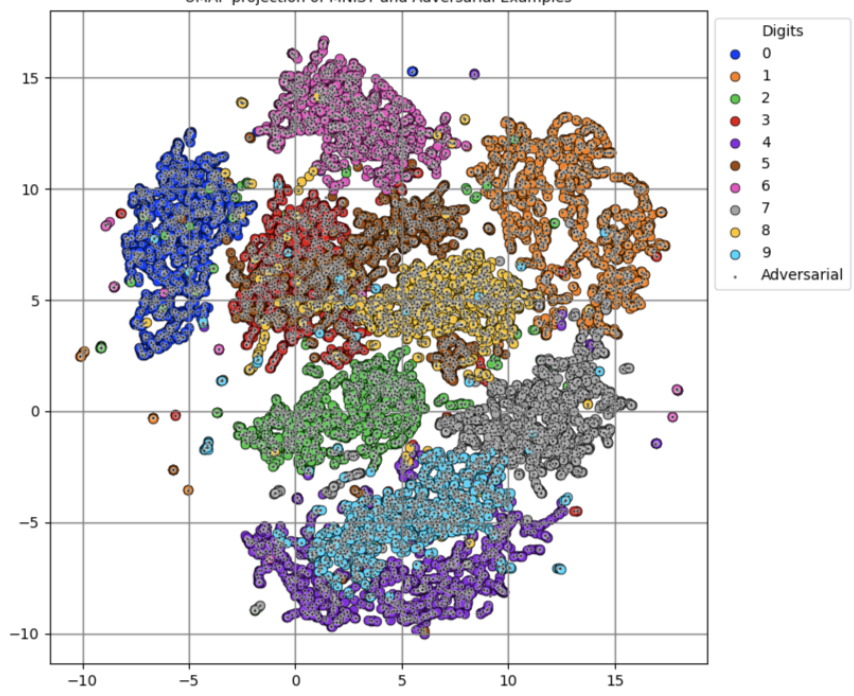
\includegraphics[width=\linewidth]{paper_images/UMAP_adv.png}
        \caption{Original and PGD attack}
        \label{fig:umap_pgd}
    \end{subfigure}%
    \hfill
    \begin{subfigure}{.28\textwidth}
        \centering
        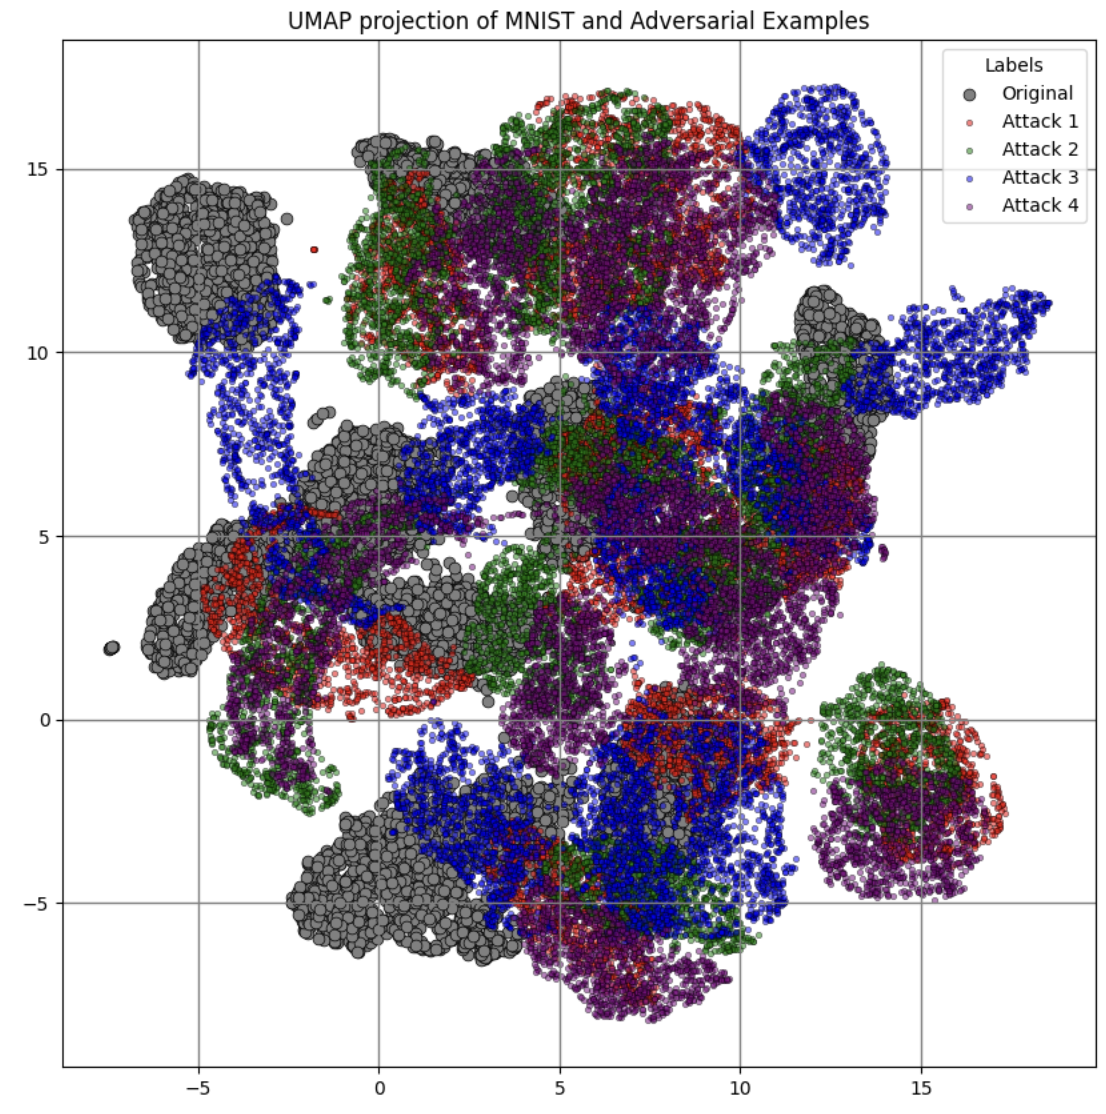
\includegraphics[width=\linewidth]{paper_images/UMAP_adversary.png}
        \caption{Original and 4 attacks}
        \label{fig:umap_additional_adv}
    \end{subfigure}
    \caption{UMAP projections illustrating the separation of digit classes within the MNIST dataset and the integration of adversarial examples. The left panel (\ref{fig:umap_original}) shows the natural clustering of MNIST digits, the middle panel (\ref{fig:umap_pgd}) overlays PGD adversarial examples, and the right panel (\ref{fig:umap_additional_adv}) displays additional adversarial examples for comparison.}
    \label{fig:umap}
\end{figure*}



To visually interpret the performance of our neural network model, we present a UMAP \cite {McInnes.}projection of the MNIST digit dataset in Figure \ref {fig:umap} , which also includes adversarial examples generated through Projected Gradient Descent (PGD) attacks. This projection delineates the ten digit classes into distinct, color-coded clusters, corresponding to the digits 0 through 9, thereby validating the model's learned pattern recognition capabilities.
Further examination of Figure.\ref {fig:umap} reveals the strategic placement of adversarial examples. These manipulated instances, designed to probe the model's classification robustness, are distributed both within and along the peripheries of the digit clusters. Unlike the well-defined groupings formed by the authentic digits, the adversarial examples demonstrate a dispersion pattern indicative of their potential to mislead the model.
The inclusion of Figure X in our analysis serves a dual purpose. Primarily, it provides a graphical representation of the insidious nature of adversarial examples, illustrating their tendency to blend seamlessly with the genuine dataset and, consequently, their ability to induce classification errors. Secondly, the figure underscores the imperative to refine our model's discriminative prowess to discern between authentic and adversarial data points effectively.
The visual evidence provided by this figure is pivotal, as it not only corroborates our findings but also highlights the emergent need to fortify neural network architectures against such adversarial intrusions. It is through this lens that we interpret the significance of our work, recognizing its contribution to advancing the security protocols inherent in machine learning applications.
\section{Stage 3: Extraction of XAI Signatures}

\subsection{Exploring Model Decision-Making}
In this stage, we concentrate on extracting explainable AI (XAI) signatures from our model. The focus is on understanding how individual input features, especially pixels, influence the model's predictions. This process is vital to discern the model's responses to both standard and adversarial inputs.

\subsection{Methodological Approach}
Our approach involved:
\begin{itemize}
    \item \textbf{Dataset Segmentation:} We selected subsets from our dataset, comprising normal examples and those modified by adversarial attacks, specifically focusing on an epsilon value of 0.2.
    \item \textbf{SHAP Deep Explainer Utilization:} We applied SHAP Deep Explainer to extract XAI signatures, revealing the significance of each pixel in the model’s predictions.
    \item \textbf{SHAP Value Calculation:} SHAP values were computed for the selected subsets to quantify the impact of each input feature on the model's output in both normal and adversarial scenarios.
\end{itemize}

\subsection{Insightful Findings}
The computed SHAP values revealed significant differences in influence patterns between normal and adversarial examples. This analysis elucidates how the model's decision-making process is affected under different input conditions.



\section{Stage 3: Extraction of XAI Signatures}

\subsection{Exploring Model Decision-Making}
In this stage, we concentrate on extracting explainable AI (XAI) signatures from our model. The focus is on understanding how individual input features, especially pixels, influence the model's predictions. This process is vital to discern the model's responses to both standard and adversarial inputs.

\subsection{Methodological Approach}
Our approach involved:
\begin{itemize}
    \item \textbf{Dataset Segmentation:} We selected subsets from our dataset, comprising normal examples and those modified by adversarial attacks, specifically focusing on an epsilon value of 0.2.
    \item \textbf{SHAP Deep Explainer Utilization:} We applied SHAP Deep Explainer to extract XAI signatures, revealing the significance of each pixel in the model’s predictions.
    \item \textbf{SHAP Value Calculation:} SHAP values were computed for the selected subsets to quantify the impact of each input feature on the model's output in both normal and adversarial scenarios.
\end{itemize}

\subsection{Insightful Findings}
The computed SHAP values revealed significant differences in influence patterns between normal and adversarial examples. This analysis elucidates how the model's decision-making process is affected under different input conditions.

\begin{figure}[h]
    \centering
    \begin{subfigure}{\columnwidth}
        \centering
        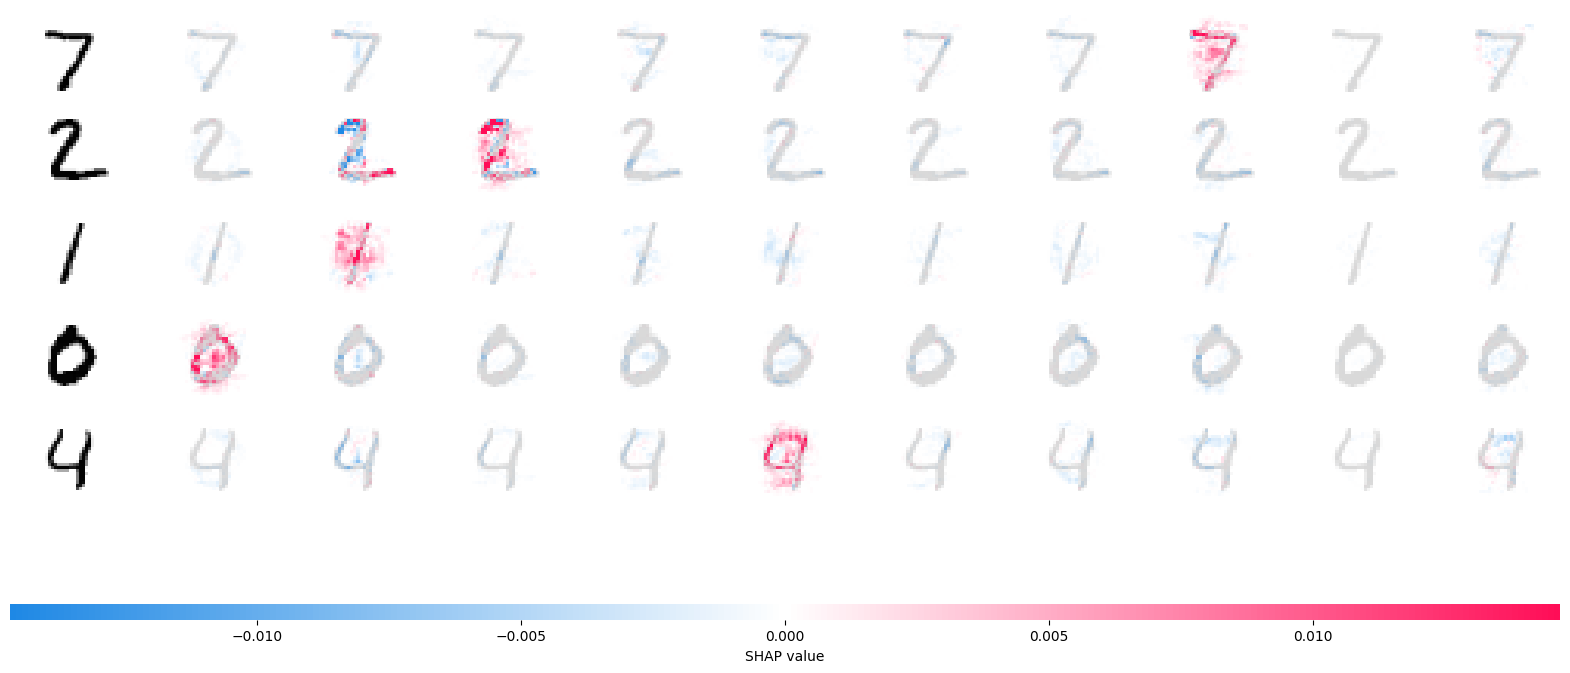
\includegraphics[width=\linewidth]{paper_images/correctshap.png}
        \caption{SHAP heatmap for correct classifications highlighting influential pixels for the model's accurate predictions.Red indicates pixels increasing model confidence, and blue shows those decreasing it in correct classifications.}
        \label{fig:correct_shap}
    \end{subfigure}
    \par\medskip % Adds space between the two subfigures
    \begin{subfigure}{\columnwidth}
        \centering
        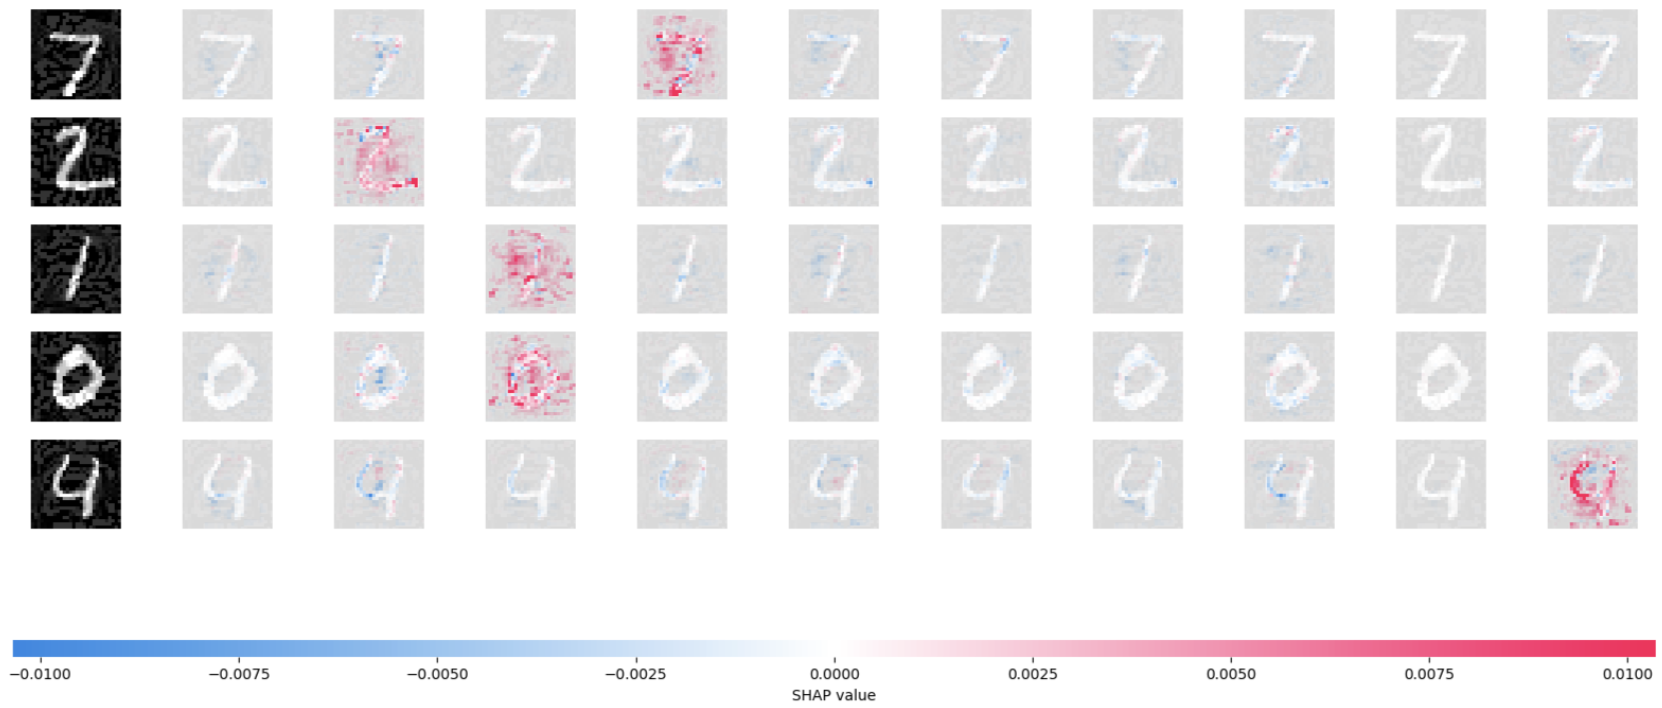
\includegraphics[width=\linewidth]{paper_images/adversarial.png}
        \caption{SHAP heatmap for adversarial samples showing how attacks distort the model's focus, leading to potential misclassifications.}
        \label{fig:adversarial}
    \end{subfigure}
    \caption{SHAP heatmaps contrast the pixel influence on the model's decisions between normal and adversarial examples, underlining the adversarial impact.}
    \label{fig:both_shap_figures}
\end{figure}


\begin{table}[h]
    \centering
    \begin{tabular}{|p{1.5cm}|p{2.5cm}|p{2.5cm}|}
    \hline
    \textbf{Aspect} & \textbf{Attack Generation} & \textbf{Attack Detection} \\ \hline
    \textbf{Objective} & Identify model vulnerabilities to change predictions. & Recognize changes in interpretation from original to adversarial instances. \\ \hline
    \textbf{Focus} & On influential features of adversarial examples. & On feature contribution differences between normal and adversarial examples. \\ \hline
    \textbf{Methodology} & Analyze SHAP values of adversarial examples. & Compare SHAP values between normal and adversarial examples. \\ \hline
    \textbf{SHAP Values Used} & From adversarial examples, indicating impactful features. & The difference in SHAP values between normal and adversarial examples. \\ \hline
    \textbf{Purpose} & Craft adversarial examples exploiting vulnerabilities. & Detect and understand adversarial attacks' effects. \\ \hline
    \textbf{Insight Gained} & Identifies model weaknesses and modification strategies. & Reveals decision-making changes due to attacks. \\ \hline
    \end{tabular}
    \caption{Key Differences Between Attack Generation and Detection Using SHAP Values}
    \label{table:attack-gen-det}
    \end{table}
    
    section{Stage 4: Identification and Validation of Critical Pixels}

    \subsection{Critical Pixel Analysis}
    Building upon the extracted SHAP values, Stage 4 focuses on identifying and validating critical pixels that significantly influence the model’s predictions. This step is crucial in understanding the model's behavior in depth and formulating strategies for enhancing robustness against adversarial attacks.
    
    \subsection{Methodological Steps}
    The process involves:
    \begin{itemize}
        \item \textbf{Identification of Critical Pixels:} Using the SHAP values, we identify pixels that play pivotal roles in the model's decision-making process.
        \item \textbf{Comparison Between Normal and Adversarial Inputs:} We compare the critical pixels between normal and adversarial inputs to understand how adversarial attacks manipulate these important features.
        \item \textbf{Empirical Validation via Visualization:} To empirically validate the significance of the identified critical pixels, we superimpose these pixels onto the original input images. This visualization offers a tangible representation of their impact on the model's decision-making process.
    \end{itemize}
    
    \subsection{Impact of Findings}
    The identification and validation of critical pixels offer profound insights into the model's vulnerabilities and strengths, guiding the development of more robust and interpretable AI systems.
    
    \begin{figure}[h]
        \centering
        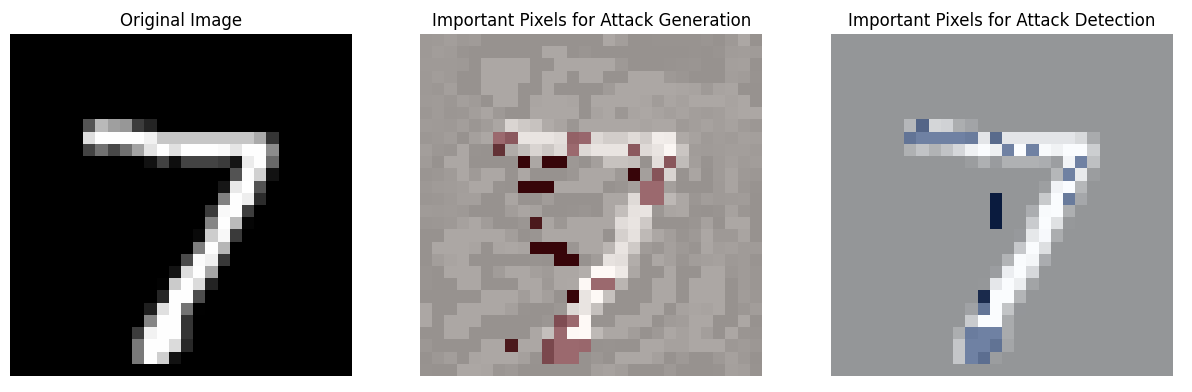
\includegraphics[width=\linewidth]{paper_images/criticalpixels.png}
        \caption{Visualization of critical pixels in adversarial samples.}
        \label{fig:adversarial}
    \end{figure}
    
    \subsection{Advancing Model Robustness}
    This stage marks a significant advancement in adversarial machine learning. By focusing on critical pixels, we unveil new avenues for developing sophisticated defense mechanisms and enhancing the interpretability and reliability of AI models in practical applications. \section{Stage 5: Binary Classification of Examples Using XAI Signatures}
    \subsection{Advancing Model Robustness (Continued)}

    \begin{table*}[t]
        \centering
        \begin{tabular}{|p{3cm}|p{6cm}|}
        \hline
        \textbf{SHAP Value Proximity to Zero} & \textbf{Interpretation} \\ \hline
        Close to Zero & 
        \begin{itemize}
        \item Feature has minimal impact on the model's prediction.
        \item Changes in the feature value do not significantly affect the prediction.
        \item Feature is considered neutral or weak in terms of prediction influence.
        \end{itemize}
        \\ \hline
        Far from Zero (Positive or Negative) & 
        \begin{itemize}
        \item Feature has a substantial impact on the model's prediction.
        \item Variations in the feature value lead to significant changes in the prediction.
        \item Feature is a strong influencer of the predicted outcome.
        \item The magnitude of the SHAP value indicates the strength of the feature's influence.
        \end{itemize}
        \\ \hline
        \end{tabular}
        \caption{Interpretations of SHAP Values Based on Proximity to Zero}
        \label{table:shap-value-interpretation}
    \end{table*}
    
    \subsection{Concluding Remarks on Stage 3 and 4}
    The findings from Stages 3 and 4 underscore the importance of interpretability in AI and its critical role in enhancing the security and reliability of machine learning models. By leveraging SHAP analysis, we have gained valuable insights into the model's decision-making process, particularly in the context of adversarial attacks. This understanding allows us to better safeguard AI systems against such manipulations and paves the way for more robust AI applications.
    
    The next section of our paper will introduce our novel approach for leveraging these critical pixels, aiming to construct a more granular line of defense against adversarial strategies. This approach promises to enhance the detection and mitigation of adversarial perturbations, marking a significant step forward in the ongoing effort to develop more secure AI systems.
    

    % In Stage 5 of our research, we focused on the development of a binary classification model that could effectively differentiate between original and adversarial examples. The crux of this stage was the utilization of XAI signatures, particularly SHAP values, instead of raw data. The choice of XAI signatures was strategic and stemmed from the need for deeper insights into the decision-making processes of neural networks. These signatures, unlike raw data, provide a nuanced understanding of feature importance and contributions, making them immensely valuable in identifying subtle manipulations in adversarial examples.

% This approach aligns with the broader objective of enhancing the interpretability and trustworthiness of deep learning models. By using XAI signatures, we aim to gain a more transparent view into how and why models make certain decisions, especially under adversarial conditions. This transparency is crucial for identifying potential vulnerabilities and strengthening the model's defenses against sophisticated attacks.

% Moreover, understanding the influence of individual features on model predictions through XAI signatures aids significantly in the research and development of more robust attack detection methods. It enables us to pinpoint which features are most exploited in adversarial attacks and thus devise more effective strategies to counter them.

% For the testing phase, we opted for a simple neural network model. This choice was deliberate; a simpler model allows for clearer interpretation of results and a more straightforward evaluation of the effectiveness of XAI signatures. It serves as a preliminary testing ground, where we can assess the viability of our approach before scaling up to more complex models. This step is essential in ensuring that our methodology is sound and effective in a controlled environment before applying it to more intricate and real-world scenarios.
% Evaluate the classification model's performance in correctly identifying adversarial attacks.

\section{Case Studies:}

This section outlines various case studies to validate the methodology.

\subsection{Case Study 1: Evaluating Model Robustness Against Different Adversarial Attacks}
The primary goal of this case study is to assess the robustness of the MNIST classification model against various adversarial attacks, including the Basic Iterative Method (BIM), Fast Gradient Sign Method (FGSM), DeepFool, and Projected Gradient Descent (PGD). The focus of the study is to compare the performance of the MNIST model before and after being subjected to these adversarial attacks. Performance is gauged by the number of misclassifications that occur at different levels of perturbation, as measured by the epsilon values. The study seeks to provide insight into the vulnerabilities of the MNIST model to different types of adversarial attacks and to gauge the effectiveness of these attacks at varying intensities.

The robust accuracy of the model against each type of attack is depicted in Figure \ref{fig:robust_accuracy_attacks}, which plots the model's accuracy as a function of epsilon, the intensity of the perturbation. The figure illustrates a clear trend of decreasing robust accuracy with increasing epsilon for all types of attacks.

\begin{figure}[ht]
    \centering
    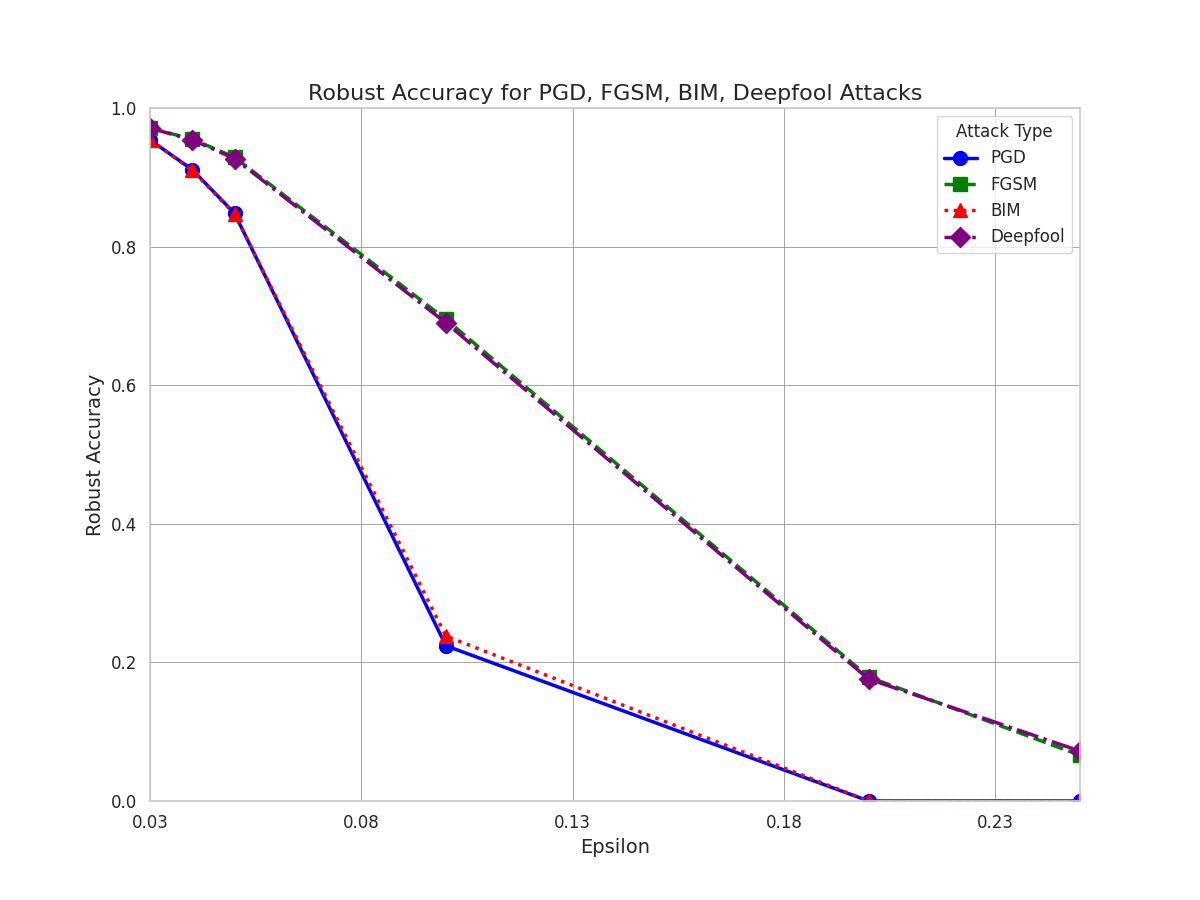
\includegraphics[width=\linewidth]{robust.png}
    \caption{Robust Accuracy for PGD, FGSM, BIM, Deepfool Attacks}
    \label{fig:robust_accuracy_attacks}
\end{figure}

As evident in the Figure. \ref{ig:robust_accuracy_attacks}, the robust accuracy for the FGSM and DeepFool attacks shows a relatively slower decline at lower epsilon values but eventually drops significantly at higher values, indicating that these attacks, while less effective at lower perturbations, can still eventually compromise the model. In contrast, BIM and PGD attacks show a more consistent and gradual decrease in robust accuracy, indicating a steady effectiveness at all levels of perturbation.

Table \ref{tab:misclassifications} provides a numerical representation of the model's vulnerabilities by listing the total number of misclassifications for each type of attack at various epsilon values. The table and the figure together give a comprehensive view of the model's performance under adversarial conditions.

\begin{table}[ht]
    \centering
    \caption{Summary of Total Misclassifications for Various Adversarial Attacks}
    \label{tab:misclassifications}
    \begin{tabular}{|l|c|c|c|c|c|c|}
    \hline
    & \multicolumn{6}{c|}{\textbf{Epsilon}} \\ \cline{2-7} 
    \multirow{-2}{*}{\textbf{Attack Type}} & \textbf{0.03} & \textbf{0.04} & \textbf{0.05} & \textbf{0.10} & \textbf{0.20} & \textbf{0.25} \\ \hline
    BIM & 451 & 881 & 1508 & 7490 & 9834 & 9834 \\ \hline
    FGSM & 284 & 440 & 702 & 2998 & 8070 & 9186 \\ \hline
    Deepfool & 289 & 449 & 713 & 3045 & 8104 & 9130 \\ \hline
    PGD & 451 & 881 & 1483 & 7616 & 9834 & 9834 \\ \hline
    \end{tabular}
\end{table}

The results underscore the need for advanced defensive strategies to improve the resilience of machine learning models against adversarial attacks. The trends identified in this case study can guide the development of such defenses, with a particular focus on the vulnerabilities exposed by BIM and PGD at lower perturbations and the delayed but eventual effectiveness of FGSM and DeepFool at higher perturbations.
\subsection{Critical Analysis of Class-Specific Metrics}

In the realm of adversarial machine learning, robust accuracy metrics and misclassification rates provide a broad overview of model performance. However, a granular understanding of adversarial impact necessitates an examination of class-specific metrics such as F1-Score, Precision, and Recall. These metrics are particularly telling, as they differentiate between false positives and false negatives—errors that carry different implications in a security context.

Our investigation extends to these class-specific metrics, meticulously compiled in the Table. \ref{table2}, which presents the F1-Score, Precision, and Recall for each class under various attack types and epsilon perturbations. The table illustrates not only the overall resilience of the model but also highlights specific class vulnerabilities, which can be obscured in more aggregated forms of analysis.

For instance, a high precision rate in the face of an attack suggests that when a model predicts a particular class, it is likely correct, albeit potentially at the expense of failing to identify all true instances (a lower recall). Conversely, a high recall with lower precision indicates a model prone to false alarms, classifying non-members as belonging to the targeted class. The F1-Score harmonizes these perspectives, providing a single metric that balances precision and recall.

A closer inspection of the table reveals that certain classes are more susceptible to specific attack types, signaling a potential need for class-conditioned defensive strategies. For example, under the FGSM attack, classes that exhibit a significant drop in F1-Score with increasing epsilon suggest that these classes are particularly sensitive to the perturbations induced by the FGSM method. This insight could guide tailored augmentation of training data or the application of class-specific defense mechanisms.

Furthermore, the disparity in robustness across classes can inform the prioritization of defense resources. Classes with markedly lower robustness metrics represent weak links in the model's armor and could benefit from focused defensive enhancements.

In summary, the detailed metrics provided in the table, when viewed in conjunction with robust accuracy trends and misclassification insights, offer a comprehensive evaluation of the model's robustness. This multifaceted assessment is instrumental in devising effective defenses against adversarial attacks, ensuring that the model not only remains accurate but also retains trustworthiness in the face of evolving adversarial challenges.


    \begin{table}[ht]
        \centering
        \resizebox{\columnwidth}{!}{%
        \begin{tabular}{cccccccccccccc}
        \toprule
        Epsilon & Class & \multicolumn{12}{c}{Metrics} \\
        \cmidrule(lr){3-14}
         & & \rotatebox{90}{F1-Score BIM} & \rotatebox{90}{F1-Score Deepfool} & \rotatebox{90}{F1-Score FGSM} & \rotatebox{90}{F1-Score PGD} & \rotatebox{90}{Precision BIM} & \rotatebox{90}{Precision Deepfool} & \rotatebox{90}{Precision FGSM} & \rotatebox{90}{Precision PGD} & \rotatebox{90}{Recall BIM} & \rotatebox{90}{Recall Deepfool} & \rotatebox{90}{Recall FGSM} & \rotatebox{90}{Recall PGD} \\
        \midrule
        0.03 & 0 & 0.9842 & 0.9872 & 0.9872 & 0.9842 & 0.9777 & 0.9817 & 0.9817 & 0.9777 & 0.9908 & 0.9928 & 0.9928 & 0.9908 \\
        0.03 & 1 & 0.9690 & 0.9788 & 0.9792 & 0.9664 & 0.9454 & 0.9601 & 0.9609 & 0.9444 & 0.9938 & 0.9982 & 0.9982 & 0.9894 \\
        0.03 & 2 & 0.9446 & 0.9675 & 0.9669 & 0.9442 & 0.9405 & 0.9694 & 0.9693 & 0.9396 & 0.9488 & 0.9656 & 0.9646 & 0.9488 \\
        0.03 & 3 & 0.9612 & 0.9778 & 0.9783 & 0.9627 & 0.9588 & 0.9749 & 0.9749 & 0.9589 & 0.9636 & 0.9808 & 0.9818 & 0.9666 \\
        0.03 & 4 & 0.9558 & 0.9717 & 0.9722 & 0.9573 & 0.9519 & 0.9692 & 0.9712 & 0.9548 & 0.9598 & 0.9742 & 0.9732 & 0.9598 \\
        0.03 & 5 & 0.9557 & 0.9715 & 0.9726 & 0.9544 & 0.9349 & 0.9571 & 0.9582 & 0.9357 & 0.9773 & 0.9864 & 0.9875 & 0.9739 \\
        0.03 & 6 & 0.9693 & 0.9796 & 0.9801 & 0.9693 & 0.9793 & 0.9860 & 0.9870 & 0.9783 & 0.9594 & 0.9733 & 0.9733 & 0.9605 \\
        0.03 & 7 & 0.9455 & 0.9682 & 0.9682 & 0.9459 & 0.9498 & 0.9682 & 0.9663 & 0.9517 & 0.9413 & 0.9682 & 0.9701 & 0.9403 \\
        0.03 & 8 & 0.9233 & 0.9464 & 0.9480 & 0.9234 & 0.9731 & 0.9807 & 0.9830 & 0.9720 & 0.8784 & 0.9144 & 0.9154 & 0.8795 \\
        0.03 & 9 & 0.9289 & 0.9550 & 0.9560 & 0.9301 & 0.9351 & 0.9619 & 0.9619 & 0.9335 & 0.9227 & 0.9482 & 0.9502 & 0.9268 \\
        0.04 & 0 & 0.9708 & 0.9826 & 0.9821 & 0.9718 & 0.9664 & 0.9766 & 0.9757 & 0.9693 & 0.9753 & 0.9887 & 0.9887 & 0.9743 \\
        0.04 & 1 & 0.9432 & 0.9708 & 0.9716 & 0.9367 & 0.9071 & 0.9464 & 0.9479 & 0.9026 & 0.9823 & 0.9965 & 0.9965 & 0.9735 \\
        0.04 & 2 & 0.8994 & 0.9461 & 0.9471 & 0.8980 & 0.8840 & 0.9424 & 0.9434 & 0.8822 & 0.9154 & 0.9498 & 0.9508 & 0.9144 \\
        0.04 & 3 & 0.9192 & 0.9596 & 0.9611 & 0.9185 & 0.9124 & 0.9577 & 0.9597 & 0.9081 & 0.9262 & 0.9616 & 0.9626 & 0.9292 \\
        0.04 & 4 & 0.9098 & 0.9568 & 0.9579 & 0.9116 & 0.8984 & 0.9529 & 0.9539 & 0.9028 & 0.9216 & 0.9607 & 0.9618 & 0.9205 \\
        0.04 & 5 & 0.8995 & 0.9546 & 0.9546 & 0.9010 & 0.8550 & 0.9320 & 0.9320 & 0.8614 & 0.9490 & 0.9785 & 0.9785 & 0.9444 \\
        0.04 & 6 & 0.9373 & 0.9698 & 0.9703 & 0.9402 & 0.9587 & 0.9804 & 0.9814 & 0.9579 & 0.9167 & 0.9594 & 0.9594 & 0.9232 \\
        0.04 & 7 & 0.9073 & 0.9512 & 0.9513 & 0.9042 & 0.9141 & 0.9521 & 0.9494 & 0.9162 & 0.9005 & 0.9502 & 0.9532 & 0.8925 \\
        0.04 & 8 & 0.8493 & 0.9163 & 0.9202 & 0.8527 & 0.9491 & 0.9704 & 0.9751 & 0.9447 & 0.7685 & 0.8679 & 0.8710 & 0.7770 \\
        0.04 & 9 & 0.8548 & 0.9304 & 0.9314 & 0.8586 & 0.8729 & 0.9371 & 0.9390 & 0.8721 & 0.8374 & 0.9238 & 0.9238 & 0.8455 \\
        0.05 & 0 & 0.9532 & 0.9750 & 0.9750 & 0.9559 & 0.9546 & 0.9686 & 0.9686 & 0.9549 & 0.9517 & 0.9815 & 0.9815 & 0.9568 \\
        0.05 & 1 & 0.9095 & 0.9534 & 0.9542 & 0.9031 & 0.8583 & 0.9169 & 0.9177 & 0.8538 & 0.9673 & 0.9929 & 0.9938 & 0.9585 \\
        0.05 & 2 & 0.8318 & 0.9189 & 0.9198 & 0.8318 & 0.8061 & 0.9118 & 0.9136 & 0.8105 & 0.8593 & 0.9262 & 0.9262 & 0.8543 \\
        0.05 & 3 & 0.8496 & 0.9311 & 0.9321 & 0.8532 & 0.8215 & 0.9260 & 0.9279 & 0.8292 & 0.8797 & 0.9363 & 0.9363 & 0.8787 \\
        0.05 & 4 & 0.8547 & 0.9300 & 0.9325 & 0.8589 & 0.8390 & 0.9143 & 0.9180 & 0.8481 & 0.8710 & 0.9463 & 0.9474 & 0.8700 \\
        0.05 & 5 & 0.8297 & 0.9208 & 0.9214 & 0.8325 & 0.7735 & 0.8825 & 0.8827 & 0.7838 & 0.8946 & 0.9626 & 0.9637 & 0.8878 \\
        0.05 & 6 & 0.8966 & 0.9533 & 0.9555 & 0.9047 & 0.9361 & 0.9701 & 0.9724 & 0.9402 & 0.8602 & 0.9370 & 0.9392 & 0.8719 \\
        0.05 & 7 & 0.8319 & 0.9297 & 0.9294 & 0.8313 & 0.8443 & 0.9320 & 0.9285 & 0.8494 & 0.8199 & 0.9273 & 0.9303 & 0.8139 \\
        0.05 & 8 & 0.7301 & 0.8671 & 0.8700 & 0.7372 & 0.8955 & 0.9566 & 0.9592 & 0.8739 & 0.6163 & 0.7928 & 0.7960 & 0.6374 \\
        0.05 & 9 & 0.7467 & 0.8838 & 0.8847 & 0.7568 & 0.7680 & 0.9069 & 0.9089 & 0.7691 & 0.7266 & 0.8618 & 0.8618 & 0.7449 \\
        0.1 & 0 & 0.5609 & 0.8876 & 0.8888 & 0.5961 & 0.7279 & 0.9032 & 0.9078 & 0.7781 & 0.4563 & 0.8726 & 0.8705 & 0.4830 \\
        0.1 & 1 & 0.3045 & 0.8518 & 0.8484 & 0.1693 & 0.3256 & 0.7599 & 0.7550 & 0.1887 & 0.2860 & 0.9691 & 0.9682 & 0.1536 \\
        0.1 & 2 & 0.2387 & 0.6409 & 0.6450 & 0.2272 & 0.2046 & 0.6216 & 0.6259 & 0.1887 & 0.2864 & 0.6614 & 0.6654 & 0.2854 \\
        0.1 & 3 & 0.2356 & 0.6673 & 0.6743 & 0.2389 & 0.2168 & 0.6361 & 0.6414 & 0.2248 & 0.2578 & 0.7017 & 0.7108 & 0.2548 \\
        0.1 & 4 & 0.3187 & 0.7195 & 0.7239 & 0.3181 & 0.2971 & 0.6844 & 0.6897 & 0.2896 & 0.3437 & 0.7585 & 0.7616 & 0.3529 \\
        0.1 & 5 & 0.2421 & 0.6843 & 0.6859 & 0.2167 & 0.2023 & 0.5861 & 0.5885 & 0.1805 & 0.3016 & 0.8220 & 0.8268 & 0.2799 \\
        0.1 & 6 & 0.3469 & 0.7821 & 0.7838 & 0.3541 & 0.3495 & 0.7862 & 0.7897 & 0.3592 & 0.3445 & 0.7781 & 0.7816 & 0.3487 \\
        0.1 & 7 & 0.2639 & 0.7425 & 0.7388 & 0.2636 & 0.2443 & 0.7002 & 0.6962 & 0.2442 & 0.2850 & 0.7899 & 0.7849 & 0.2852 \\
        0.1 & 8 & 0.1718 & 0.5624 & 0.5684 & 0.1669 & 0.1545 & 0.5486 & 0.5554 & 0.1630 & 0.1908 & 0.5767 & 0.5836 & 0.1823 \\
        0.1 & 9 & 0.1869 & 0.6064 & 0.6067 & 0.1825 & 0.1791 & 0.5892 & 0.5903 & 0.1749 & 0.2007 & 0.6307 & 0.6312 & 0.1960 \\
        0.15 & 0 & 0.1935 & 0.7615 & 0.7528 & 0.1575 & 0.1092 & 0.4804 & 0.4791 & 0.1029 & 0.4565 & 0.9307 & 0.9198 & 0.0896 \\
        0.15 & 1 & 0.0709 & 0.6661 & 0.6512 & 0.0337 & 0.0471 & 0.4160 & 0.4070 & 0.0240 & 0.0512 & 0.9329 & 0.9247 & 0.0160 \\
        0.15 & 2 & 0.0679 & 0.4026 & 0.3763 & 0.0367 & 0.0379 & 0.2362 & 0.2215 & 0.0195 & 0.0349 & 0.7530 & 0.7172 & 0.0295 \\
        0.15 & 3 & 0.0761 & 0.5076 & 0.4773 & 0.0381 & 0.0407 & 0.2717 & 0.2545 & 0.0238 & 0.0371 & 0.6646 & 0.6317 & 0.0250 \\
        0.15 & 4 & 0.1186 & 0.5514 & 0.5331 & 0.0652 & 0.0781 & 0.2929 & 0.2822 & 0.0485 & 0.1094 & 0.6452 & 0.6279 & 0.0863 \\
        0.15 & 5 & 0.0650 & 0.4053 & 0.3756 & 0.0365 & 0.0364 & 0.2327 & 0.2200 & 0.0190 & 0.0345 & 0.7612 & 0.7270 & 0.0501 \\
        0.15 & 6 & 0.1199 & 0.5737 & 0.5454 & 0.0700 & 0.0716 & 0.3386 & 0.3220 & 0.0521 & 0.1091 & 0.6117 & 0.5798 & 0.0883 \\
        0.15 & 7 & 0.0862 & 0.4992 & 0.4735 & 0.0435 & 0.0453 & 0.2627 & 0.2486 & 0.0272 & 0.0418 & 0.6993 & 0.6636 & 0.0306 \\
        0.15 & 8 & 0.0392 & 0.2970 & 0.2852 & 0.0233 & 0.0235 & 0.1733 & 0.1641 & 0.0142 & 0.0213 & 0.5872 & 0.5625 & 0.0186 \\
        0.15 & 9 & 0.0418 & 0.2780 & 0.2645 & 0.0248 & 0.0247 & 0.1542 & 0.1460 & 0.0136 & 0.0224 & 0.6013 & 0.5675 & 0.0203 \\
        0.2 & 0 & 0.0703 & 0.6920 & 0.6672 & 0.0430 & 0.0385 & 0.4683 & 0.4532 & 0.0262 & 0.0273 & 0.9781 & 0.9657 & 0.0159 \\
        0.2 & 1 & 0.0247 & 0.4637 & 0.4494 & 0.0125 & 0.0140 & 0.3394 & 0.3267 & 0.0065 & 0.0073 & 0.9782 & 0.9684 & 0.0035 \\
        0.2 & 2 & 0.0262 & 0.2206 & 0.2057 & 0.0121 & 0.0126 & 0.1392 & 0.1307 & 0.0062 & 0.0066 & 0.8852 & 0.8351 & 0.0029 \\
        0.2 & 3 & 0.0277 & 0.3064 & 0.2876 & 0.0141 & 0.0147 & 0.1912 & 0.1797 & 0.0071 & 0.0074 & 0.8694 & 0.8184 & 0.0036 \\
        0.2 & 4 & 0.0414 & 0.3921 & 0.3736 & 0.0219 & 0.0226 & 0.2323 & 0.2189 & 0.0107 & 0.0111 & 0.8492 & 0.8054 & 0.0052 \\
        0.2 & 5 & 0.0237 & 0.2087 & 0.1929 & 0.0115 & 0.0119 & 0.1276 & 0.1192 & 0.0058 & 0.0061 & 0.8889 & 0.8524 & 0.0030 \\
        0.2 & 6 & 0.0464 & 0.4479 & 0.4291 & 0.0242 & 0.0250 & 0.2796 & 0.2648 & 0.0118 & 0.0122 & 0.8348 & 0.7989 & 0.0061 \\
        0.2 & 7 & 0.0330 & 0.2947 & 0.2750 & 0.0166 & 0.0171 & 0.1900 & 0.1779 & 0.0084 & 0.0087 & 0.8596 & 0.8159 & 0.0042 \\
        0.2 & 8 & 0.0167 & 0.1629 & 0.1540 & 0.0083 & 0.0085 & 0.1239 & 0.1170 & 0.0054 & 0.0057 & 0.7417 & 0.7070 & 0.0036 \\
        0.2 & 9 & 0.0149 & 0.1434 & 0.1339 & 0.0076 & 0.0077 & 0.1121 & 0.1052 & 0.0050 & 0.0053 & 0.7470 & 0.7096 & 0.0029 \\
        0.25 & 0 & 0.0175 & 0.3467 & 0.3191 & 0.0090 & 0.0088 & 0.2839 & 0.2619 & 0.0049 & 0.0047 & 0.9914 & 0.9714 & 0.0024 \\
        0.25 & 1 & 0.0092 & 0.1963 & 0.1750 & 0.0049 & 0.0048 & 0.1289 & 0.1161 & 0.0025 & 0.0024 & 0.9883 & 0.9725 & 0.0013 \\
        0.25 & 2 & 0.0076 & 0.1060 & 0.0940 & 0.0032 & 0.0031 & 0.0708 & 0.0633 & 0.0017 & 0.0016 & 0.9912 & 0.9881 & 0.0010 \\
        0.25 & 3 & 0.0082 & 0.1311 & 0.1175 & 0.0034 & 0.0033 & 0.0900 & 0.0804 & 0.0018 & 0.0017 & 0.9849 & 0.9747 & 0.0010 \\
        0.25 & 4 & 0.0142 & 0.1885 & 0.1677 & 0.0059 & 0.0057 & 0.1228 & 0.1106 & 0.0029 & 0.0028 & 0.9634 & 0.9715 & 0.0015 \\
        0.25 & 5 & 0.0065 & 0.1045 & 0.0923 & 0.0030 & 0.0029 & 0.0702 & 0.0620 & 0.0016 & 0.0015 & 0.9906 & 0.9888 & 0.0010 \\
        0.25 & 6 & 0.0176 & 0.2197 & 0.1954 & 0.0075 & 0.0073 & 0.1170 & 0.1040 & 0.0027 & 0.0026 & 0.9635 & 0.9732 & 0.0014 \\
        0.25 & 7 & 0.0134 & 0.1649 & 0.1473 & 0.0057 & 0.0056 & 0.0943 & 0.0842 & 0.0023 & 0.0022 & 0.9705 & 0.9731 & 0.0013 \\
        0.25 & 8 & 0.0044 & 0.0710 & 0.0645 & 0.0020 & 0.0019 & 0.0429 & 0.0387 & 0.0010 & 0.0010 & 0.9621 & 0.9569 & 0.0005 \\
        0.25 & 9 & 0.0040 & 0.0644 & 0.0576 & 0.0018 & 0.0017 & 0.0382 & 0.0343 & 0.0009 & 0.0008 & 0.9648 & 0.9571 & 0.0004 \\              
        \bottomrule
    \end{tabular}
    }
    \caption{Class-Specific Performance Metrics under Adversarial Attacks: This table delineates the F1-Score, Precision, and Recall for each MNIST class (0 through 9) across a spectrum of adversarial attacks at varying levels of epsilon perturbations. The metrics provide insights into the differential impact of each attack (BIM, Deepfool, FGSM, and PGD) on the classifier's ability to robustly identify each digit, underscoring the nuanced vulnerabilities and resilience of the model on a class-by-class basis.}

    \label{table2}
    \end{table}


    \subsection{Case Study 2: Validation of Identified Critical Pixels}

    To ascertain the significance of the critical pixels identified  as discussed in Section VI through our methodology for both attack 
    generation and detection, we conducted a rigorous statistical validation employing a two-sample t-test. 
    This pivotal validation step serves as a means to underscore the crucial role played by these critical pixels
    in shaping the decision-making process of our machine learning model.
    
    Our approach involved a comprehensive examination of SHAP values, with specific emphasis placed on those
     related to attack detection. These SHAP values are instrumental in unraveling the inner workings of our model, 
     shedding light on the pixels that exert a significant influence over its predictions.
      To streamline the analysis, we categorized these SHAP values into two distinct groups: 
      those corresponding to critical pixels and those associated with non-critical pixels, based on a set of 
      indices derived from our methodology.Figure \ref{fig:bar_chart} illustrates a bar chart comparing the means of these two groups, 
    demonstrating the difference in mean SHAP values for 'Critical' and 'Non-Critical' pixels. 
    This visual representation is an essential component of our analysis.Figure \ref{fig:histograms} presents histograms of SHAP values, providing a closer look at the 
    distribution of SHAP values for both 'Critical' and 'Non-Critical' pixels. These histograms assist 
    in understanding the data distribution and its impact on statistical tests.
    
    The essence of our validation hinges on the statistical comparison of these two groups. 
    The two-sample t-test, a widely recognized method for discerning meaningful distinctions 
    between two sets of data, yielded significant results. The computed t-statistic, registering at 
    a noteworthy value of 11.5968, in conjunction with an exceedingly low p-value of $1.34 \times 10^{-30}$, 
    furnishes compelling evidence. These statistical indicators (as shown in Figures \ref{fig:bar_chart} and 
    \ref{fig:histograms}) affirm that critical pixels indeed play a substantial role in influencing our model's 
    behavior, both in terms of generating adversarial attacks and detecting them.
    
    \begin{figure}[h]
        \centering
        \begin{subfigure}{.45\textwidth}
            \centering
            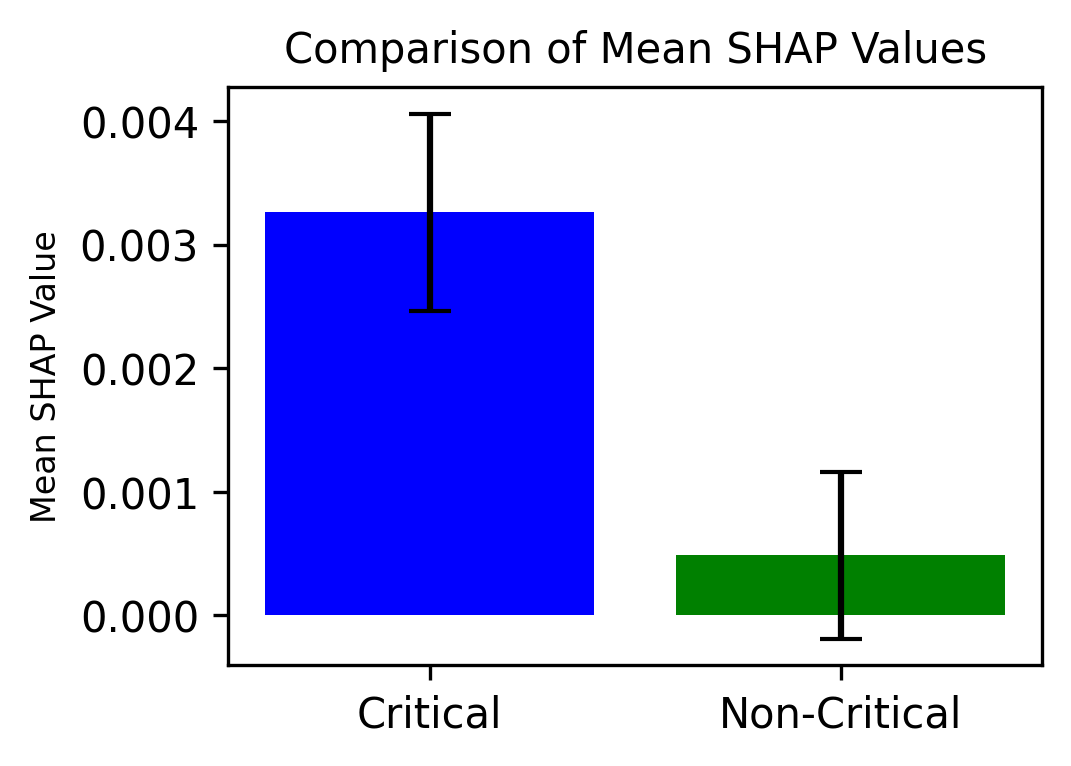
\includegraphics[width=\linewidth]{paper_images/bar_chart.png}
            \caption{Comparison of Mean SHAP Values. The bar chart illustrates a comparison between the mean SHAP values for 'Critical' and 'Non-Critical' groups. Error bars represent standard deviations. This graph is essential for assessing the significance of the differences between these groups.}
            \label{fig:bar_chart}
        \end{subfigure}
        \par\medskip % Adds space between the two subfigures
        \begin{subfigure}{\columnwidth}
            \centering
            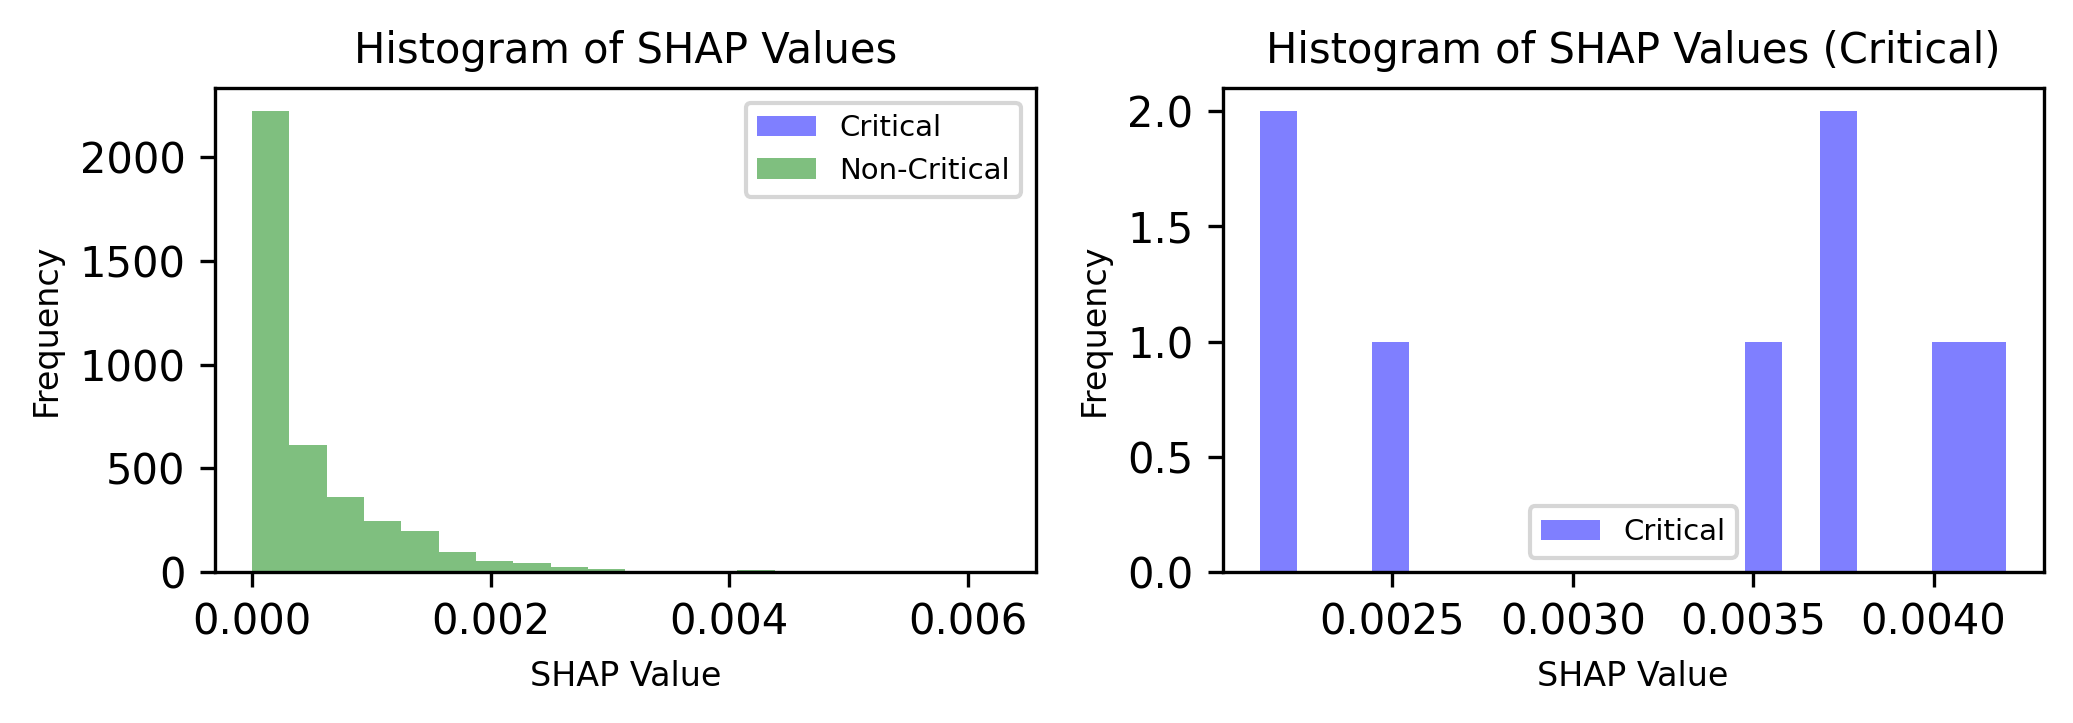
\includegraphics[width=\linewidth]{paper_images/histograms.png}
            \caption{Histograms of SHAP Values. In the left subplot, the histogram depicts the distribution of SHAP values for both 'Critical' (in blue) and 'Non-Critical' (in green) groups. The right subplot zooms in on the 'Critical' group's SHAP values. These histograms provide insights into the data distribution and its impact on statistical tests}
            \label{fig:histograms}
        \end{subfigure}
        \caption{ SHAP values into critical and non-critical groups}
    \end{figure}
    \subsection{Case Study 3: Deep Dive into the Model's Penultimate Layer}
\textbf{Objective:} Gain insights into the model's internal processing by examining the penultimate layer. \\
\textbf{Key Focus:} Explore feature processing changes in response to adversarial examples. \\
\textbf{Outcome:} Deeper understanding of the model's internal mechanisms.

\subsection{Case Study 4: Binary Classification Using XAI Signatures}

In our experimental analysis focusing on binary classification using XAI signatures, the model trained over 10 epochs demonstrated progressive improvement, culminating in training and validation accuracies of 82.21% and 78.05%, respectively. Notably, the model's performance on the test data reached an accuracy of 73.08%, reflecting its capability but also suggesting potential areas for refinement. The precision and recall metrics were reasonably balanced across both classes, with the model showing a slight preference for classifying adversarial examples (class 1.0). The confusion matrix revealed a fair distribution between true positives and negatives, and false positives and negatives, underscoring the model's proficiency in distinguishing between original and adversarial examples.

A key highlight of the experiment was the AUC score of 0.84, indicating a strong ability of the model to differentiate between the classes, a crucial aspect in the context of adversarial machine learning. This score not only reflects the model's current effectiveness but also guides future enhancements to increase its reliability and robustness against sophisticated adversarial attacks.

\section{Future Directions and Challenges:}

F\section{Conclusion:}

\begin{thebibliography}{01}
    \bibitem{Akhtar}
    Akhtar, N., Mian, A. (2018). Threat of Adversarial Attacks on Deep Learning in Computer Vision: A Survey. IEEE Access. Link
    \bibitem{Dong}
    Dong, Y., Liao, F., Pang, T., Su, H., Zhu, J., Hu, X.,  Li, J. (2017). Boosting Adversarial Attacks with Momentum. IEEE/CVF Conference on Computer Vision and Pattern Recognition. Link
    \bibitem{Lee}
    Lee, K., Lee, K., Lee, H.,  Shin, J. (2018). A Simple Unified Framework for Detecting Out-of-Distribution Samples and Adversarial Attacks. ArXiv. Link
    \bibitem{Morris}
    Morris, J. X., Lifland, E., Yoo, J. Y., Grigsby, J., Jin, D.,  Qi, Y. (2020). TextAttack: A Framework for Adversarial Attacks, Data Augmentation, and Adversarial Training in NLP. Conference on Empirical Methods in Natural Language Processing. Link
    \bibitem{Croce}
    Croce, F., Hein, M. (2020). Reliable evaluation of adversarial robustness with an ensemble of diverse parameter-free attacks. International Conference on Machine Learning. Link
    \bibitem{Zhou}
    Zhou, X., Liang, W., Li, W., Yan, K., Shimizu, S.,  Wang, K. (2022). Hierarchical Adversarial Attacks Against Graph-Neural-Network-Based IoT Network Intrusion Detection System. IEEE Internet of Things Journal. Link
    \bibitem{Entezari}
    Entezari, N., Al-Sayouri, S. A., Darvishzadeh, A.,  Papalexakis, E. (2020). All You Need Is Low (Rank): Defending Against Adversarial Attacks on Graphs. Web Search and Data Mining. Link

\bibitem{McInnes.}
	L. McInnes, J. Healy, and J. Melville, “UMAP: Uniform Manifold Approximation and Projection for Dimension Reduction,” ArXiv e- prints, Feb. 2018.
   

\end{thebibliography}

\end{document}
